\chapter{Results and Analysis}\label{chap_results}
\minitoc

%%%%%%%%%%%%%%%%%%%%%%%%%%%%%%%%%% Intro %%%%%%%%%%%%%%%%%%%%%%%%%%%%%%%%%%%%%%%
The results obtained here were taken over the course of a month at the Femtosecond Spectroscopy Laboratory. All figures unless mentioned otherwise were generated by me.

Original datasets were recorded as plain text files with whitespace separated columns as depicted in figure \ref{fig_datafile}. Column two is the relative position of the stage (in steps), column three is the signal count, column four is the reference count, and column five is the ratio between the two. Column one is always null.

\begin{figure}[h]
\begin{Verbatim}[frame=single,fontfamily=courier,fontsize=\small]
0  2700  38.000   3656.000  0.010
0  2750  51.000   3618.000  0.014
0  2800  48.000   3575.000  0.013
0  2850  53.000   3624.000  0.015
0  2900  39.000   3706.000  0.011
0  2950  37.000   3431.000  0.011
0  3000  43.000   3556.000  0.012
0  3050  70.000   3360.000  0.021
0  3100  167.000  3459.000  0.048
0  3150  243.000  3243.000  0.075
0  3200  317.000  3387.000  0.094
0  3250  230.000  3158.000  0.073
0  3300  151.000  3173.000  0.048
0  3350  80.000   3339.000  0.024
\end{Verbatim}
\caption[Example data file.]{Example data file, from left to right: null column, position, signal counts, reference counts, ratio between the two.\label{fig_datafile}}
\end{figure}

Most of the figures in this chapter were created by plotting the ratio of the signals (normalized counts) against the position of the platform. The position of the platform is in steps and was multiplied by 0.625 to yield micrometers, the unit used in the figures. 

%%%%%%%%%%%%%%%%%%%%%%%%%%%%%%%%%% Linear Transmission %%%%%%%%%%%%%%%%%%%%%%%%%%%%%%%%%%%%%%%
\section{Linear Transmission}
Figure \ref{fig_transmission} shows the transmission curves for all samples. Substrate absorption dominates in the 200 - 350 nm range. The spectrophotometer switches lamps at 350 nm which accounts for the abrupt drop in all samples. The two gold samples demonstrate plasmon resonance around 530 nm that coincides with a drop in transmittance. This result coincides with literature \cite{schaadt2005enhanced, lin2005one}.

Strangely, the transmission curve for the silicon nanoparticles is almost completely flat. When physically compared with the samples described in \cite{PhysRevB.84.165316}, this sample appears to be a much darker gray color. Likewise, the transmission spectra of those samples do present an absorption region while this sample does not.

\begin{figure}[h]
\centering
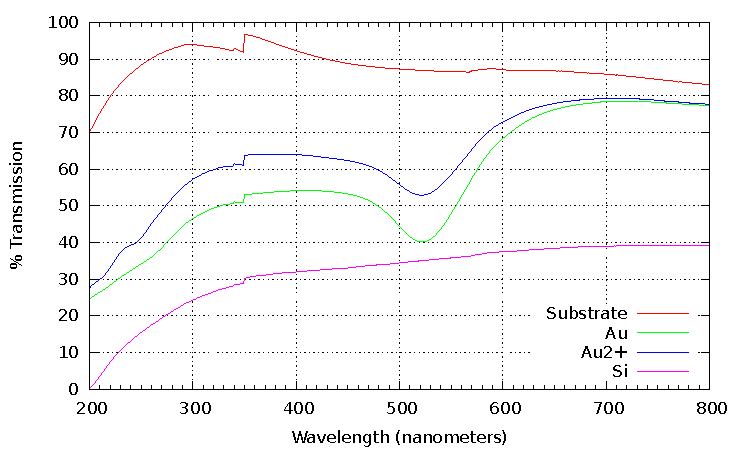
\includegraphics[width=\textwidth]{results/linear_transmission}
\caption{Transmission curves from the three samples and substrate.\label{fig_transmission}}
\end{figure}

%%%%%%%%%%%%%%%%%%%%%%%%%%%%%%%%%% Reference Samples %%%%%%%%%%%%%%%%%%%%%%%%%%%%%%%%%%%%%
\section{Reference Glass and Substrate}
Initial measurements were taken on the glass and substrate samples mentioned in section \ref{chap_setup_glass}. Both glass and substrate present typical behavior when compared to previous measurements taken by the Femtosecond Spectroscopy group.

\subsection{Ellipsometry}
The ellipsometric results shown in figure \ref{fig_sub_ellip} for the substrate are consistent with the data in \cite{PhysRevB.84.165316}. The graphs depict the polarization change represented as an amplitude ratio, $\Psi$, and and the phase difference, $\Delta$. These were the clearest results for this measurement of the four different samples. 

\begin{figure}[h]
  \centering
  \subfloat[Graph for $\Psi$.\label{fig_sub_ellip_1}]{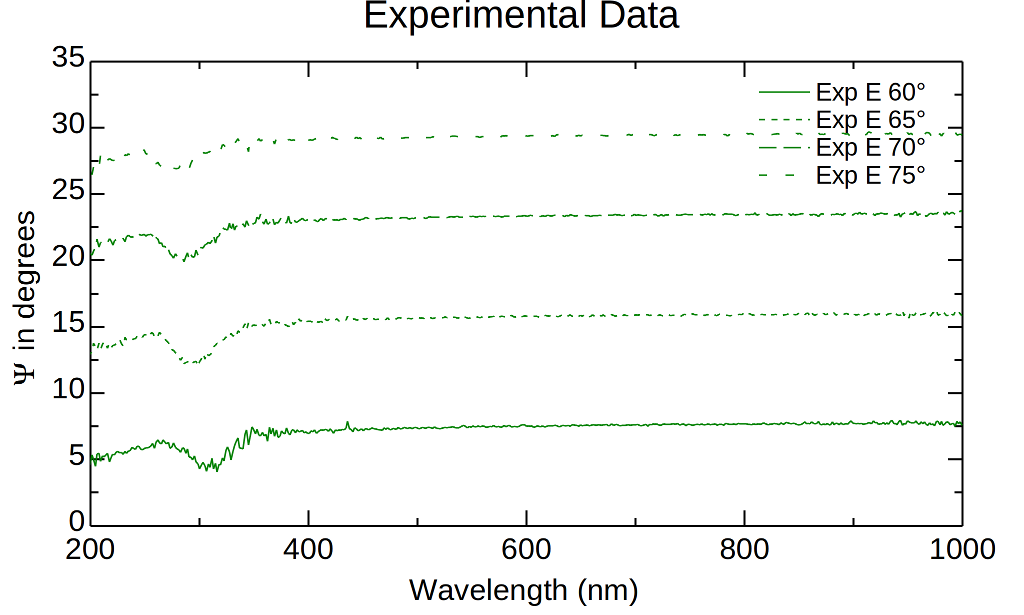
\includegraphics[width=0.5\textwidth]{results/sub_ellipsometry_1}}  
  \subfloat[Graph for $\Delta$.\label{fig_sub_ellip_2}]{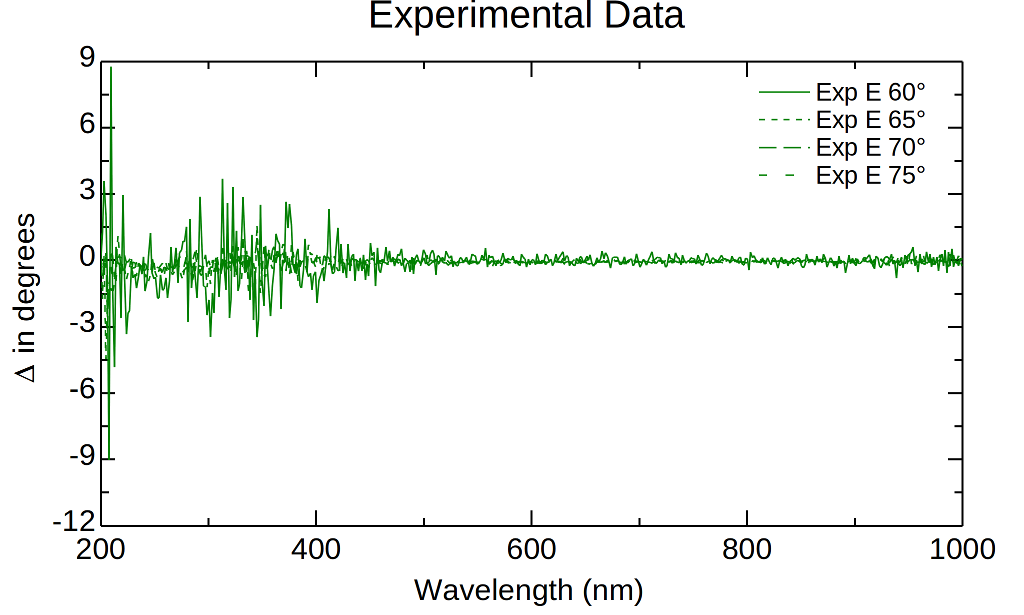
\includegraphics[width=0.5\textwidth]{results/sub_ellipsometry_2}}
  \caption[Substrate ellipsometry.]{Substrate ellipsometry. Graphs courtesy of Junwei Wei.}
  \label{fig_sub_ellip}
\end{figure}

\subsection{XP2SHG and XP2SFG}\label{chap_results_sub_shg}
Figures \ref{fig_glass_shg} and \ref{fig_glass_sfg} both show two distinguishable peaks for the glass reference sample in both SHG and SFG configurations. One peak corresponds to the two beam spots coinciding on the front surface, then on the back and are due to the interference between fields at both surfaces and phase mismatching \cite{sun2005nonresonant}. These peaks are very similar since this sample has no nanoparticles on it. 

\begin{figure}[h]
\centering
\subfloat[XP2SHG signal.\label{fig_glass_shg}]{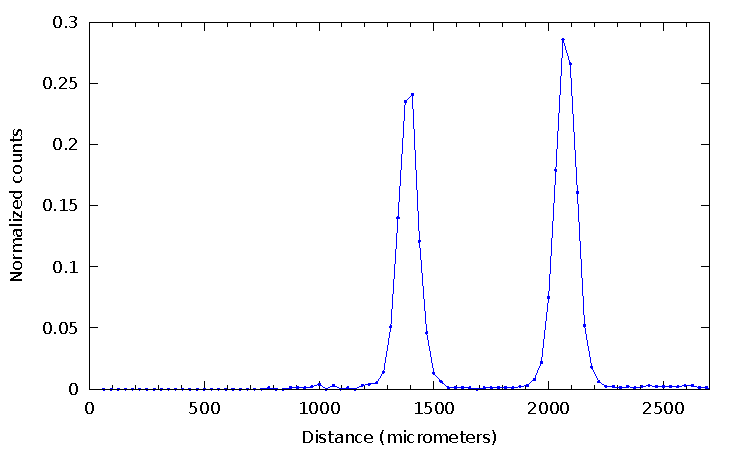
\includegraphics[width=0.5\textwidth]{results/glass_shg}}
\subfloat[XP2SFG signal from 550 and 800 nm beams.\label{fig_glass_sfg}]{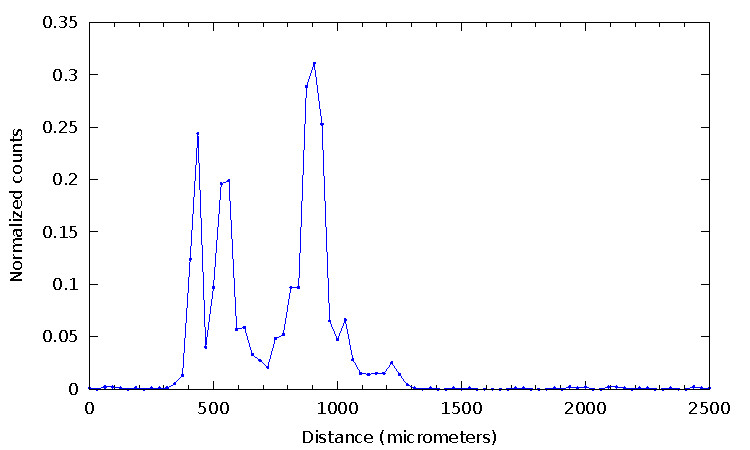
\includegraphics[width=0.5\textwidth]{results/glass_sfg_550+800}}
\caption{SHG and SFG Signals from reference glass.}
\end{figure}

The misshapen first peak of figure \ref{fig_glass_sfg} is due to the difficulty of properly filtering both beams in SFG. Filtering SHG is easier because there are only two wavelengths involved: the fundamental and the signal. There are three in SFG -- the fundamental, the idler, and the signal. Filtering the SFG setup requires at least two distinct filters, one for the 800 nm fundamental and one for the 550 nm idler. This is why both peaks appear to be broader than in figure \ref{fig_glass_shg}, and also accounts for the discrepancy in the sample width as can be measured by the distance between peaks. The real sample width is closer to figure \ref{fig_glass_shg}, at around 700 micrometers.

The substrate shows very similar peaks, as we can see in figures \ref{fig_sub_sfg1} and \ref{fig_sub_sfg2}. Two peaks are clearly resolved when the NOPA wavelength is at 520 nm. The 550 nm beam is more energetic, which explains the additional signal in between the peaks in figure \ref{fig_sub_sfg2}. This signal is emitted from the bulk material and is due to white light generation. Both figures clearly depict the sample width to be around 500 micrometers in thickness. All these observations are consistent with the literature reviewed in section \ref{chap_theory_xp2}.

\begin{figure}[h]
\centering
\subfloat[XP2SFG signal from 520 and 800 nm.\label{fig_sub_sfg1}]{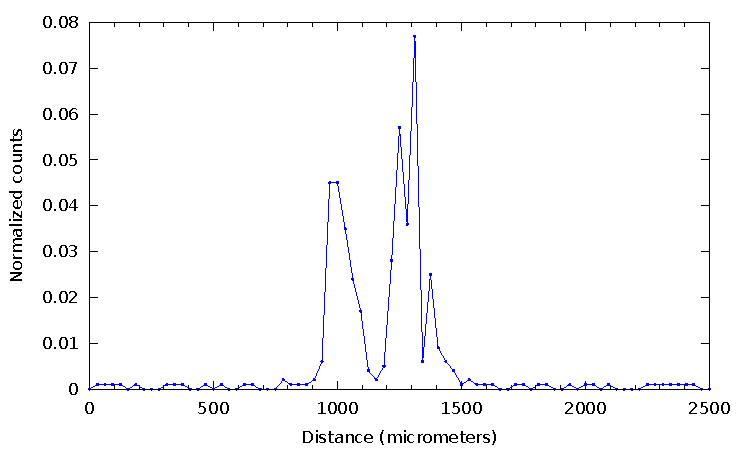
\includegraphics[width=0.5\textwidth]{results/sub_sfg_520+800}}
\subfloat[XP2SFG signal from 550 and 800 nm.\label{fig_sub_sfg2}]{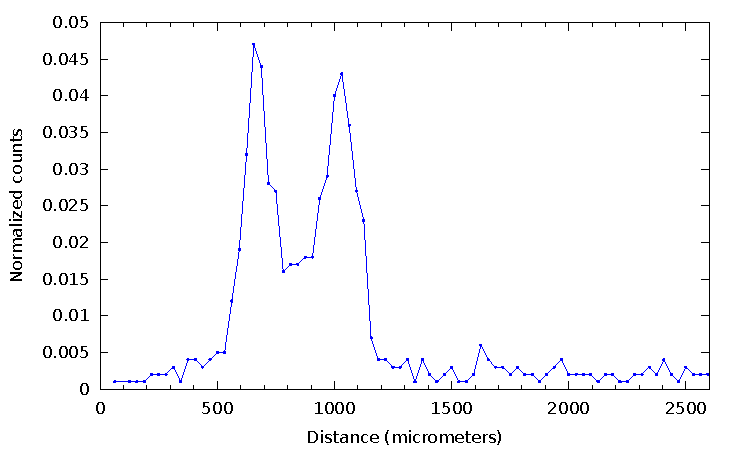
\includegraphics[width=0.5\textwidth]{results/sub_sfg_550+800}}
\caption{SHG and SFG Signals from substrate.}
\end{figure}


%%%%%%%%%%%%%%%%%%%%%%%%%%%%%%%%%% Gold Samples %%%%%%%%%%%%%%%%%%%%%%%%%%%%%%%%%%%%%
\section{Gold Nanoparticles}
The gold nanoparticles were previously described in section \ref{chap_setup_gold}. They underwent the same measurements as the reference samples. Unfortunately these samples present considerable wear and tear that can easily seen with the naked eye. Scratches and other imperfections mar the surface. These imperfections cause a significant amount of scattering. This problem persisted throughout the entire experiment and led to the significant setup change I mentioned at the end of chapter \ref{chap_setup}.

\subsection{Ellipsometry}
Ellipsometric measurements where taken for the gold nanoparticles in the same way as the reference samples. Both sides were analyzed for completeness since it is not always apparent which side has the nanoparticles.

Data from ellipsometry cannot be directly interpreted -- a model must be constructed that fits the data and in the process determines several optical constants, the film thickness, and characteristics of surface. However, the raw data almost always produces well defined curves. The data obtained here is both noisy and unclear. What little distinguishable features that figures \ref{fig_au_ellip_front_1} and \ref{fig_au_ellip_back_1} have are identical to those of the substrate as seen in figure \ref{fig_sub_ellip_1}.

Junwei Wei speculated that the scattering problem is the most likely reason for the unreadable ellipsometry data. Most literature on ellipsometry talk about opaque samples -- these samples are transparent and have a much smaller signal by reflection. He concluded that the data produced here would not yield any relevant results if used with the modeling algorithms.

\begin{figure}[h]
  \centering
  \subfloat[Graph for $\Psi$.]{\label{fig_au_ellip_front_1}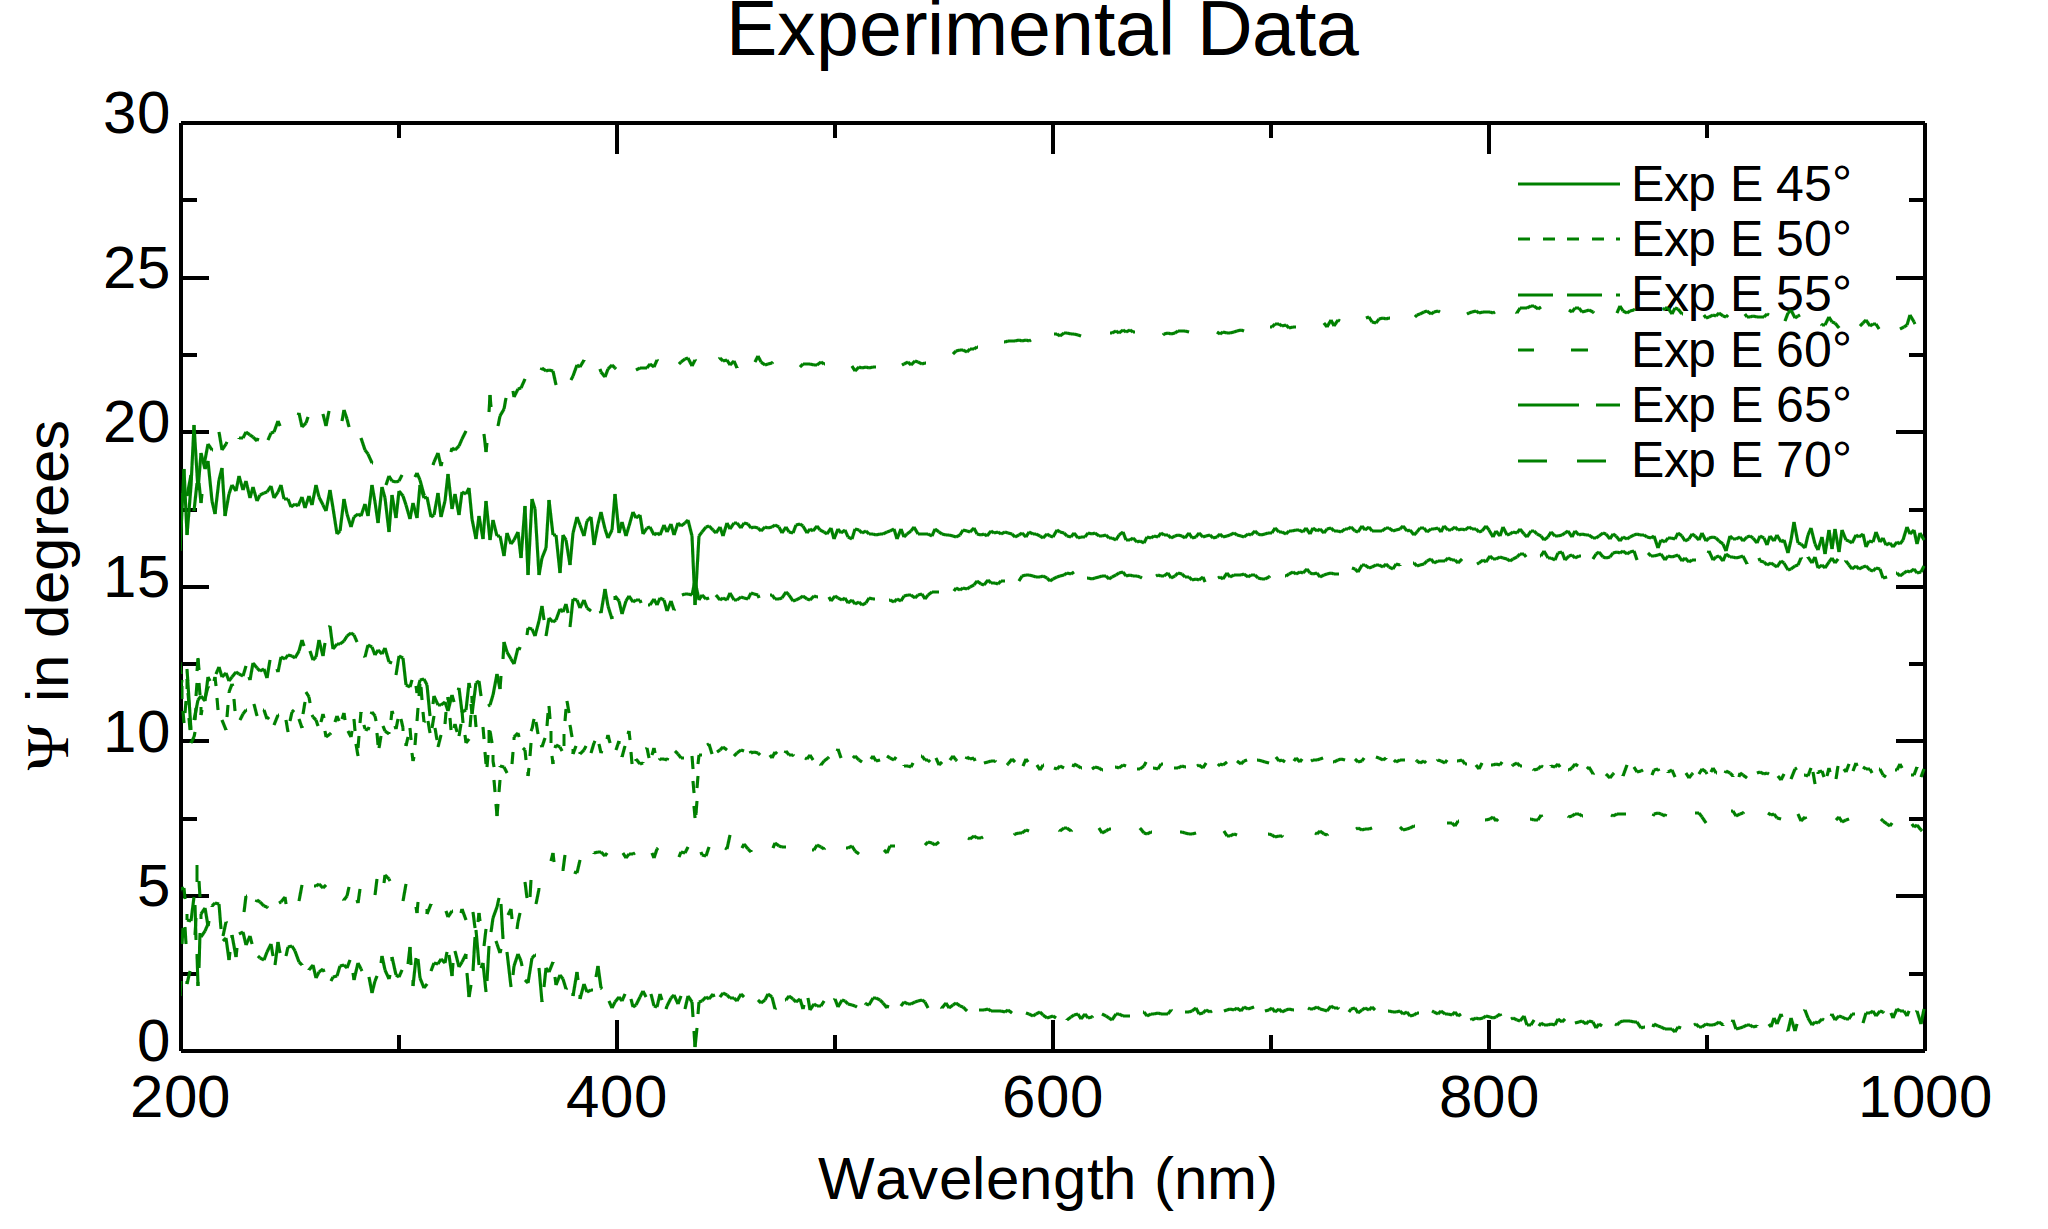
\includegraphics[width=0.5\textwidth]{results/au_ellipsometry_front_1}}  
  \subfloat[Graph for $\Delta$.]{\label{fig_au_ellip_front_2}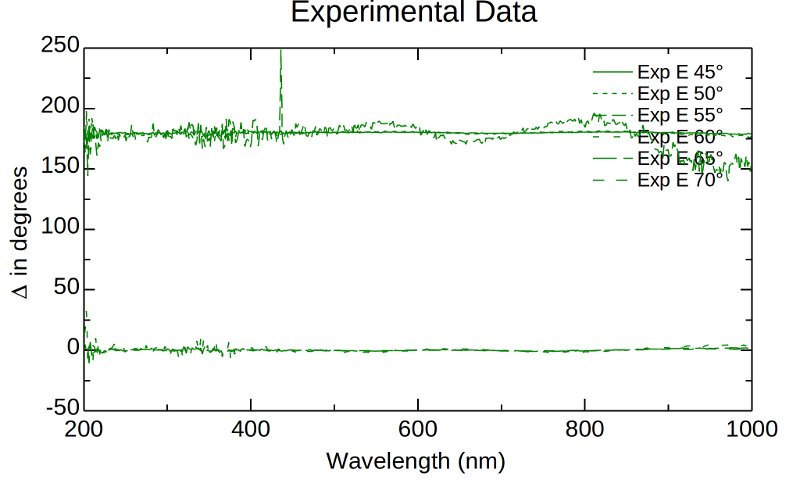
\includegraphics[width=0.5\textwidth]{results/au_ellipsometry_front_2}}
  \caption[Au ellipsometry, front side.]{Au ellipsometry, front side. Graphs courtesy of Junwei Wei.\label{fig_au_ellip_front}}
\end{figure}

\begin{figure}[h]
  \centering
  \subfloat[Graph for $\Psi$.]{\label{fig_au_ellip_back_1}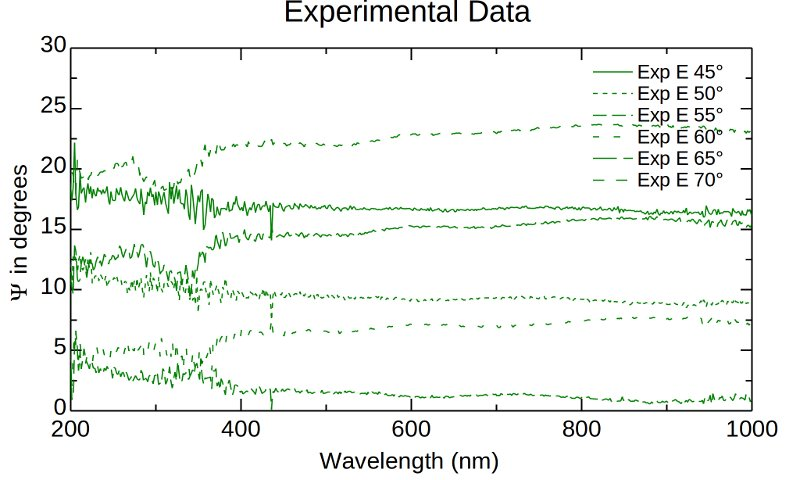
\includegraphics[width=0.5\textwidth]{results/au_ellipsometry_back_1}}  
  \subfloat[Graph for $\Delta$.]{\label{fig_au_ellip_back_2}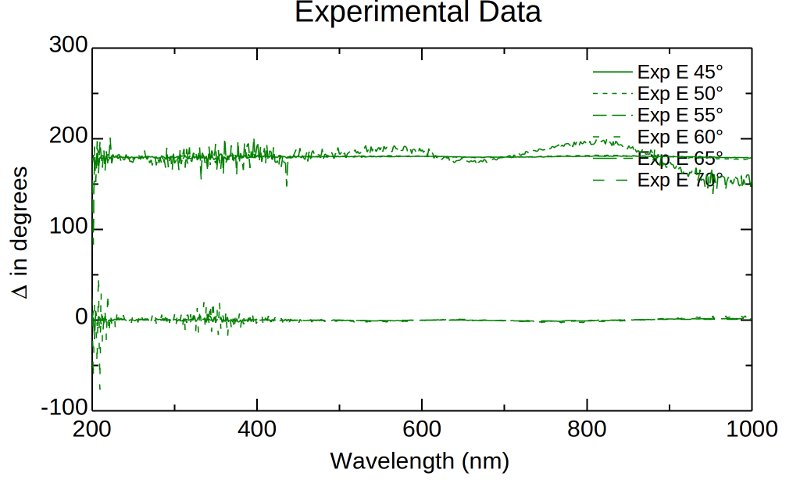
\includegraphics[width=0.5\textwidth]{results/au_ellipsometry_back_2}}
  \caption[Au ellipsometry, reverse side.]{Au ellipsometry, reverse side. Graphs courtesy of Junwei Wei.\label{fig_au_ellip_back}}
\end{figure}

The ellipsometry data for the ionic gold sample (figure \ref{fig_au2+_ellip}) is virtually identical to the others.

\begin{figure}[h]
  \centering
  \subfloat[Graph for $\Psi$.]{\label{fig_au2+_ellip_1}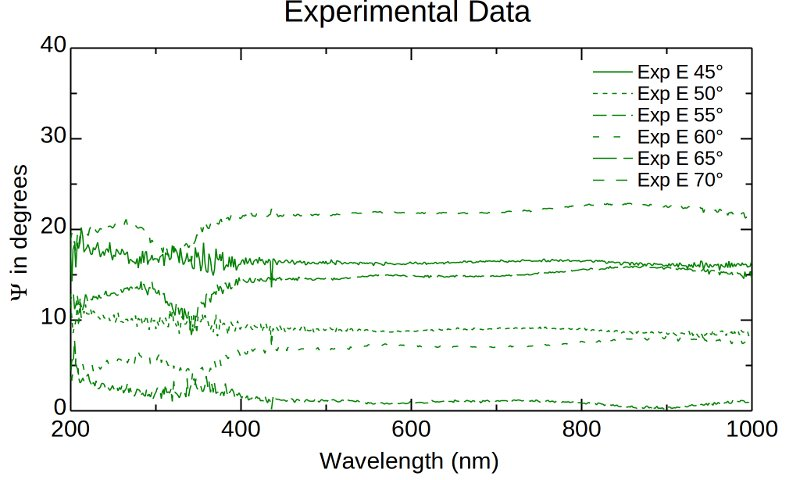
\includegraphics[width=0.5\textwidth]{results/au2+_ellipsometry_1}}  
  \subfloat[Graph for $\Delta$.]{\label{fig_au2+_ellip_2}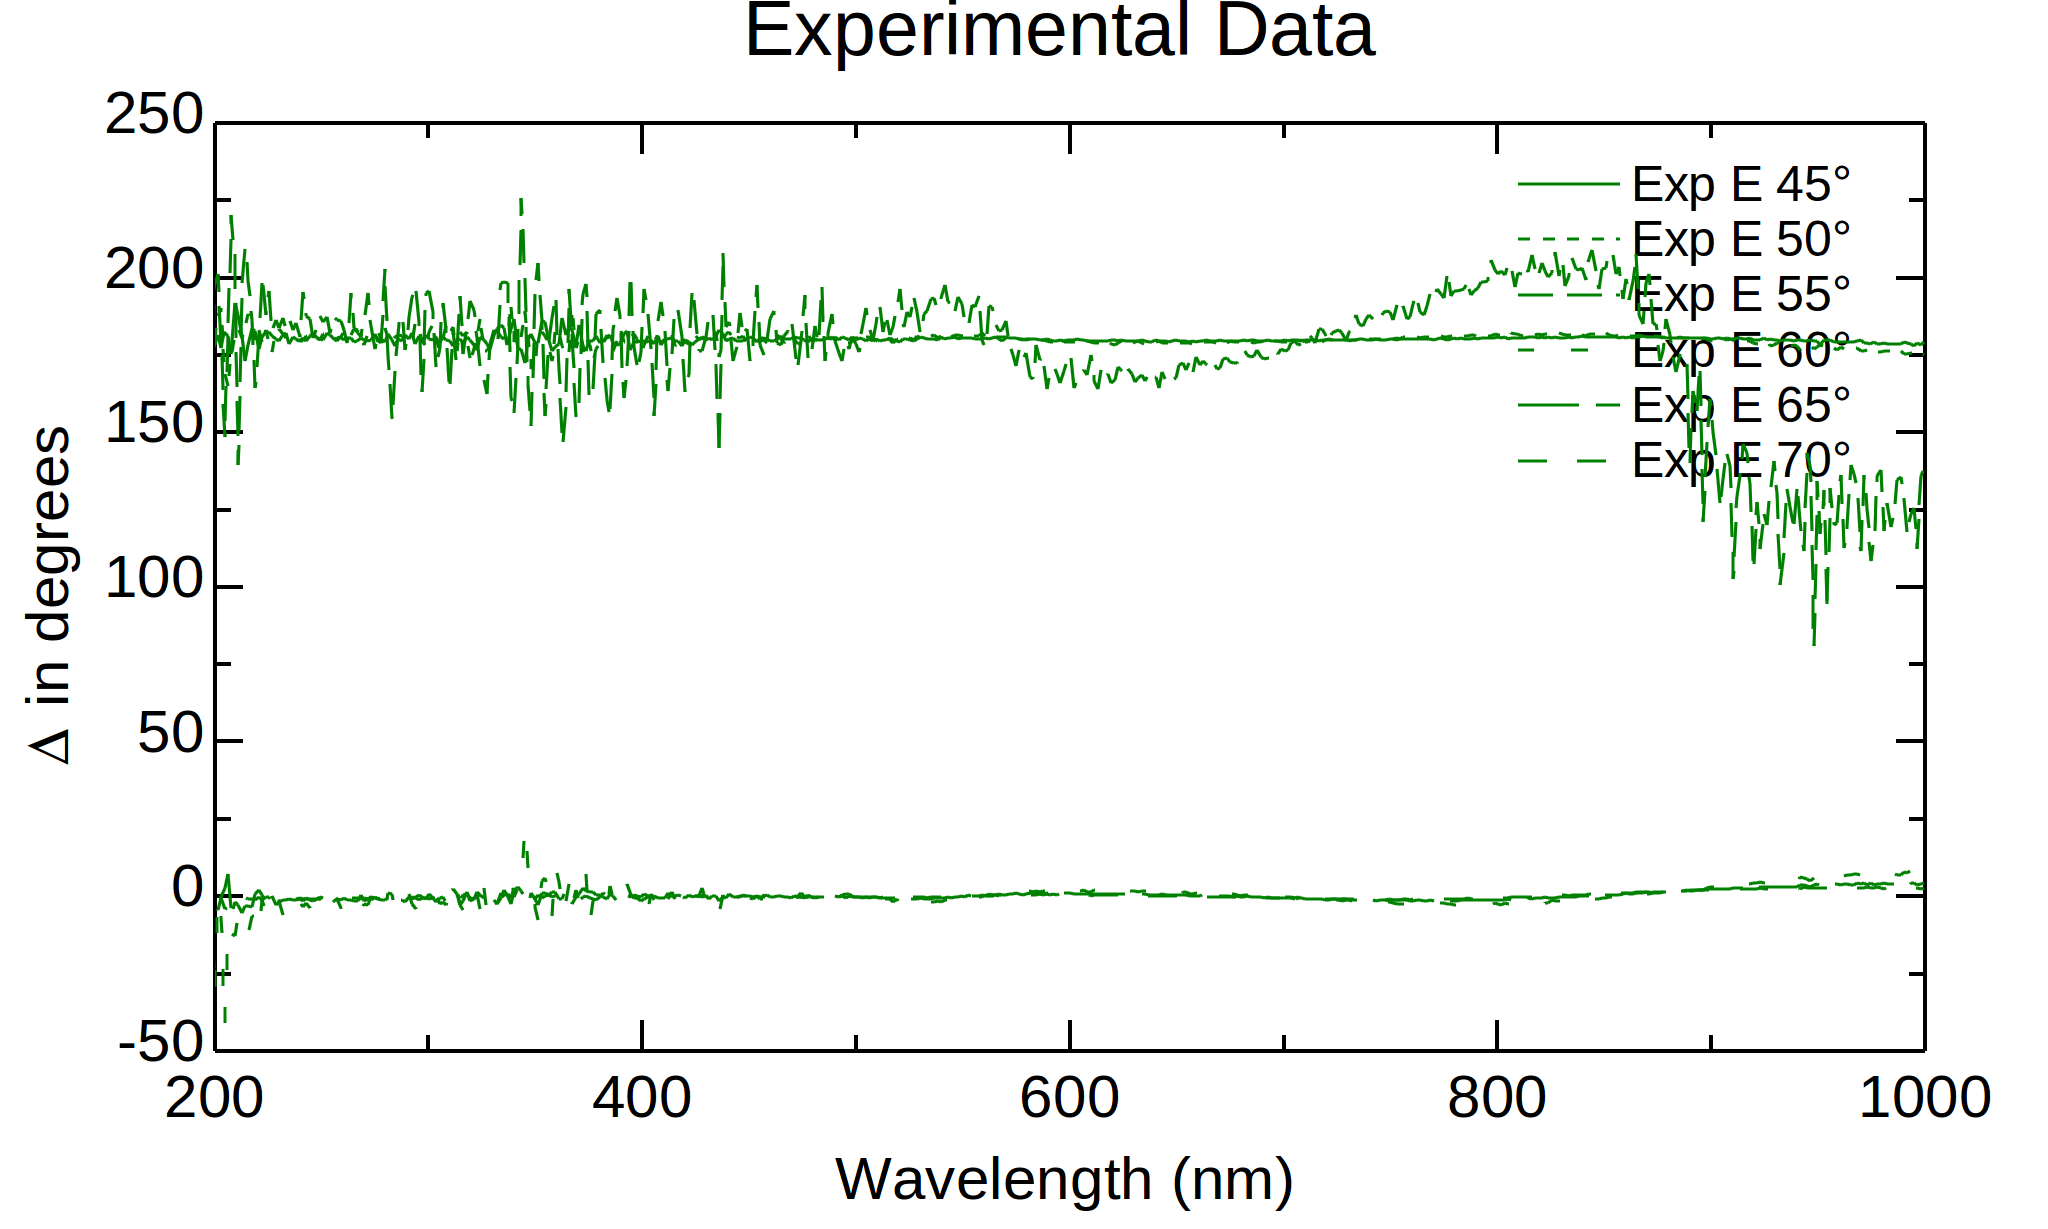
\includegraphics[width=0.5\textwidth]{results/au2+_ellipsometry_2}}
  \caption[Au$^{2+}$ ellipsometry.]{Au$^{2+}$ ellipsometry. Graphs courtesy of Junwei Wei.\label{fig_au2+_ellip}}
\end{figure}

Zhang et al. \cite{zhang2003spectroscopic} detail similar measurements on thin films of gold nanoparticles. Their results show very distinct curves with a clear absorption region. The samples in that article have an absorption band slightly higher than these, centered around 580 nm. These measurements are very noisy compared to the curves depicted there.

\subsection{Filter Tests}
The first thing that is needed is confirmation that the samples can produce a strong second-order signal. A quick filter test is the easiest way to confirm this. The monochromator is scanned across most of the PMT range and the counts are recorded. For figure \ref{fig_filter_no}, we removed all filters from the detectors and blocked the 800 nm beam. Two very prominent peaks corresponding to SHG signal produced in the sample and NOPA were detected with very high intensities. The broadness of the SHG peak (left) is most likely due to white light generation in the crystal for these high intensities.

\begin{figure}[h]
\centering
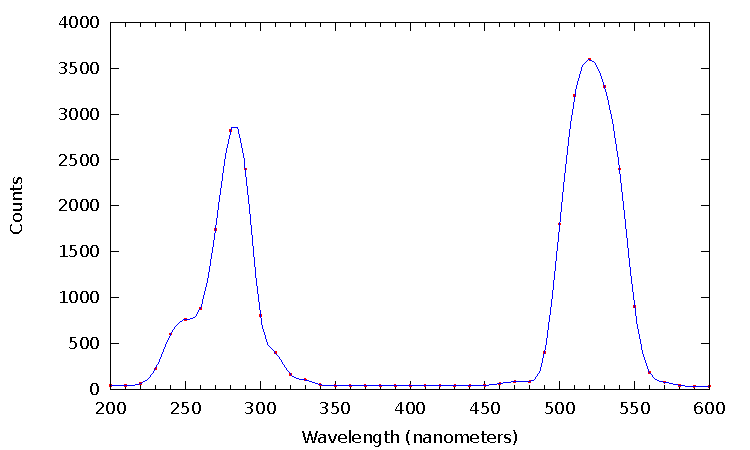
\includegraphics[width=0.875\textwidth]{results/au_nofilter}
\caption{Spectrum from gold sample, no filters.\label{fig_filter_no}}
\end{figure}

We then placed different filters in front of the sample detector. The UG5 filter blocks most light in the 500 - 600 nm range. Placing two in front of the detector block out most of the NOPA signal, as seen in figure \ref{fig_filter_half}. We placed an additional OG515 filter for figure \ref{fig_filter_all}, which blocks out everything below 500 nm and yields only noise. This basic test demonstrates that the sample is indeed capable of producing single beam SHG.

\begin{figure}[h]
\centering
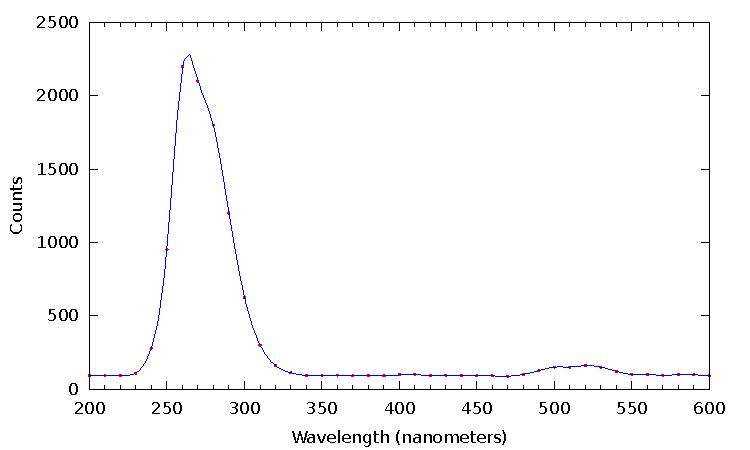
\includegraphics[width=0.875\textwidth]{results/au_ug5+ug5_2}
\caption[Spectrum from gold sample, with filters.]{Spectrum from gold sample, two UG5 filters.\label{fig_filter_half}}
\end{figure}

\begin{figure}[H]
\centering
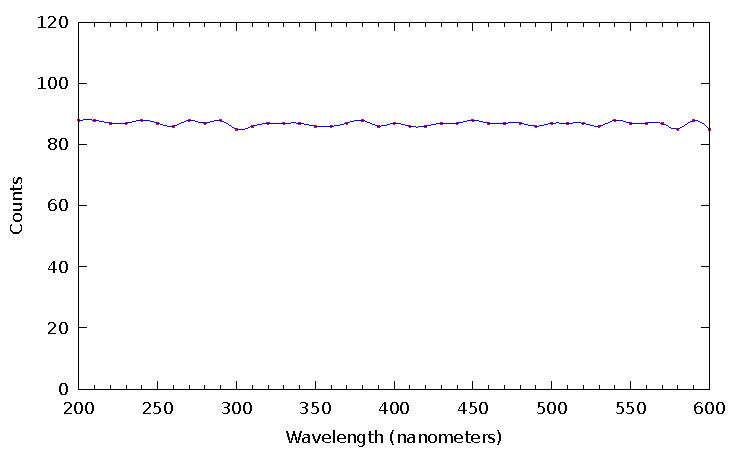
\includegraphics[width=0.875\textwidth]{results/au_og515+ug5+ug5}
\caption[Spectrum from gold sample, with more filters.]{Spectrum from gold sample, two UG5 and one OG515 filters.\label{fig_filter_all}}
\end{figure}

\subsection{XP2SHG Measurements}
Figure \ref{fig_au_shg_narrow} depicts two very well resolved peaks for the Au sample. A higher intensity peak before a lower one means that the nanoparticles were facing the incoming beams in the entrance position. This pattern occurs because the SHG signal is strongest at the nanoparticle surface; for entrance position, the nanoparticles produce SHG first. That signal goes through the remaining glass and is detected. The sample continues to move and SHG is produced on the unimplanted surface, but at a smaller intensity.

A big problem arises when comparing with the substrate data -- how can we distinguish the substrate from the nanoparticles? At first glance, both figures \ref{fig_au_shg_narrow} and \ref{fig_glass_shg} share similarities. We learned that other groups solved this problem (section \ref{chap_theory_xp2}) by taking three separate Z-scans. Naturally, we needed to take data from the samples at both entrance and exit positions.

\begin{figure}[h]
\centering
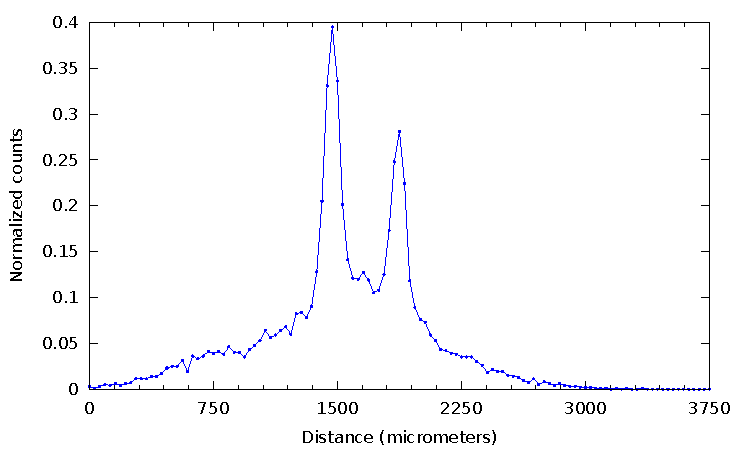
\includegraphics[width=0.9\textwidth]{results/au_shg_narrow}
\caption[Resolved XP2SHG peaks.]{Resolved XP2SHG peaks for gold nanoparticles. Entry side.\label{fig_au_shg_narrow}}
\end{figure}

Figure \ref{fig_au_shg_whitelight} shows the sample in the exit position, with the nanoparticles facing the detector. The order of the peaks is reversed from figure \ref{fig_au_shg_narrow}. For this case, the SHG signal produced by the nanoparticles is free to travel straight to the detector without crossing the substrate. This figure also demonstrates what happens when input intensity is increased slightly. The idea was that increasing the incoming beam would cause a stronger SHG emission from the nanoparticles; instead, white light generation was observed. This is observed in the elongated bump towards the right side of the graph which corresponds to outside the second surface of the sample. Even though the beams were no longer spatially overlapped inside or on the surface of the sample, their intensity was still sufficiently strong to create white light -- perhaps also an indication of some single beam SHG.

\begin{figure}[h]
\centering
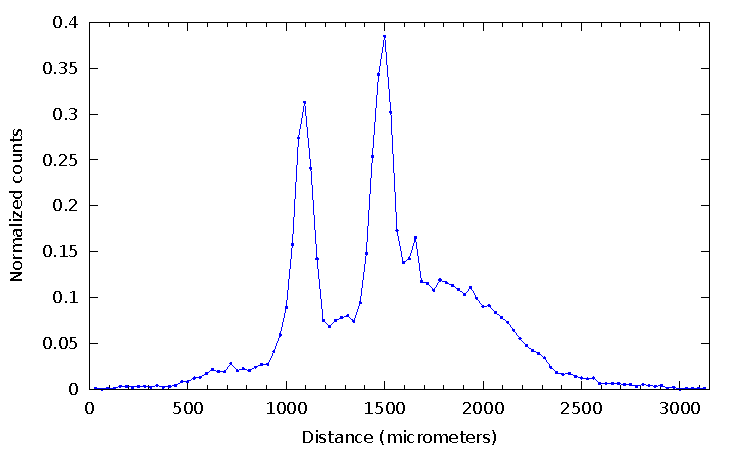
\includegraphics[width=0.85\textwidth]{results/au_shg_whitelight}
\caption[White light generation, gold sample.]{White light generation in gold sample, exit position. Note how counts do not go to zero even when the overlapped beams are outside the sample.\label{fig_au_shg_whitelight}}
\end{figure}

\begin{figure}[H]
\centering
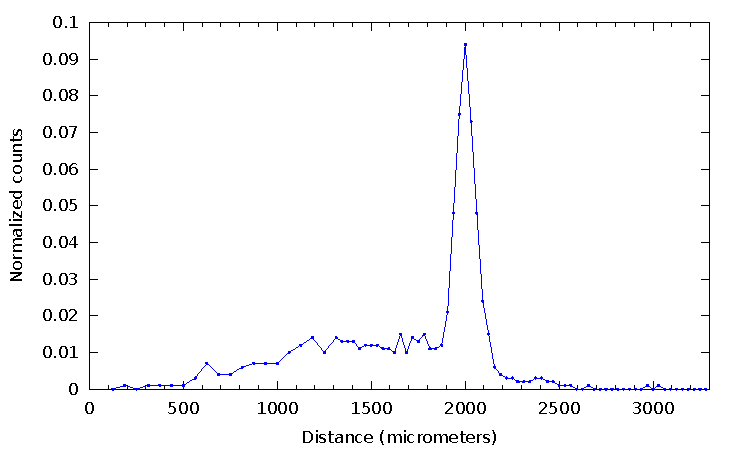
\includegraphics[width=0.85\textwidth]{results/au_shg_best}
\caption{Weaker XP2SHG signal, gold sample.\label{fig_au_shg_best}}
\end{figure}

Lowering the input intensity presented it own share of problems. Figure \ref{fig_au_shg_best} shows SHG emission using one tenth of the previous intensity. The obvious difference is that it lacks an entire peak (also note scale). However, this figure is probably the best data run for the SHG setup; although it lacks a peak, the fact that it was able to radiate at the low intensities is a good case for only nanoparticle contribution without the substrate.

It is easy to read from the previous figures that the sample width is around 500 micrometers, confirming the observation in section \ref{chap_results_sub_shg}.

\subsection{XP2SFG Measurements}
Once the setup had been switched from XP2SHG to XP2SFG, we tested the sample again. Figure \ref{fig_au_sfg_best} represents the best SFG data run with the gold sample. Again, it is impossible to distinguish the substrate contribution from the nanoparticles.

SFG measurements for the gold samples were very inconsistent compared to SHG even though the setup had been properly tested. Figure \ref{fig_sfg_au2+} is a clear example of this. A very noisy signal is present even at relatively high intensities. The two peaks can no longer be resolved.

\begin{figure}[h]
\centering
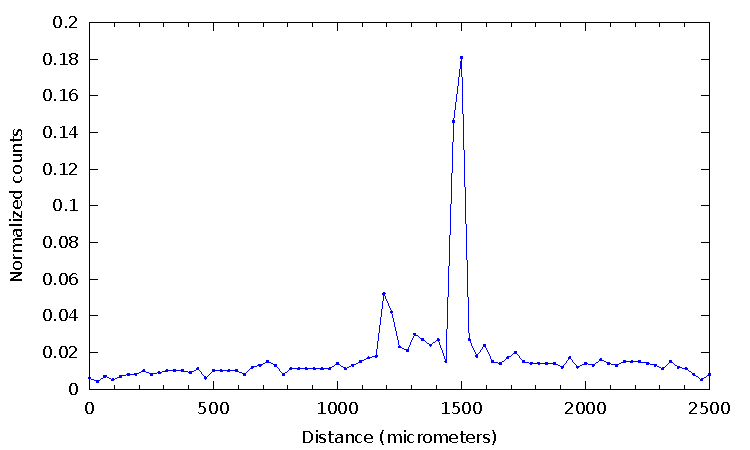
\includegraphics[width=\textwidth]{results/au_sfg_550+800_best}
\caption{Best results for gold sample with XP2SFG setup.\label{fig_au_sfg_best}}
\end{figure}

Scattering was still present even with SFG and an increased beam angle. Most of the data for SFG produced graphs similar to \ref{fig_au_sfg_whitelight}. There is clearly only white light emission with no distinguishable features. This figure in particular was taken with similar input intensities as figure \ref{fig_au_sfg_best} but does not have a similar shape at all.

\begin{figure}[h]
\centering
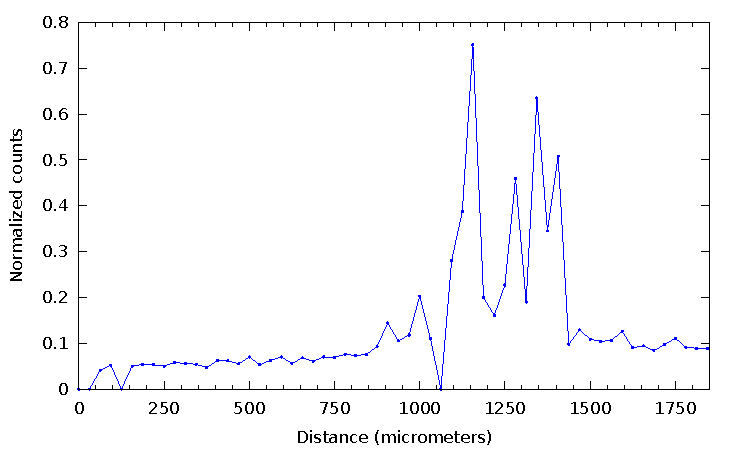
\includegraphics[width=0.9\textwidth]{results/au2+_sfg_520+800}
\caption[Noisy XP2SFG signal for Au$^{2+}$ sample.]{Very noisy XP2SFG signal for Au$^{2+}$ sample. Possible white light emission.\label{fig_sfg_au2+}}
\end{figure}

\subsection{Analysis}
Results where ambiguous at best. The bad physical condition of the samples led to the scattering problem that we never fully resolved. It still presented a problem even after increasing the beam angle and switching from the XP2SHG to the XP2SFG configuration. Shutting down all irises did alleviate the problem, but not enough to be able to present unequivocal data.

Using the 550 nm beam to match the plasmon resonance of the sample became problematic because single beam SHG started to occur, regardless of being in the cross beam geometry.

\begin{figure}[h]
\centering
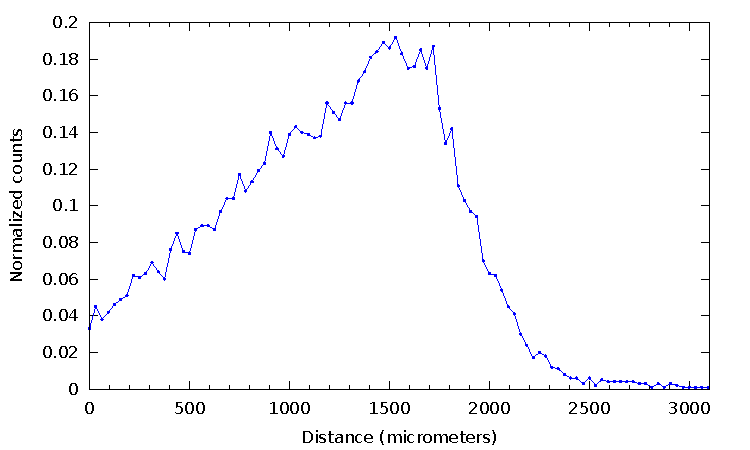
\includegraphics[width=\textwidth]{results/au_sfg_560+800_whitelight}
\caption[White light emission, gold sample.]{White light emission with 560 NOPA beam, gold sample.\label{fig_au_sfg_whitelight}}
\end{figure}

The samples also had a relatively small tolerance for white light emission especially with the XP2SFG setup. Reducing the 800 nm beam with a 0.8 optical density (OD) neutral density filter yielded no emission distinguishable from the substrate. Going down to 0.7 OD there was white light generation, as depicted in figure \ref{fig_au_sfg_whitelight}. Effectively working in a 0.1 OD difference was challenging. Adjusting beam sizes became the best means for controlling the input intensity -- a solution far from optimal. 

This becomes especially apparent when comparing with the figures of references \cite{PhysRevB.84.165316} and \cite{wirth2008second} which elaborate on the models used to determine the different response coefficients based on the empirical data. I asked Junwei Wei about the data we were obtaining and he said that it varied too much from run to run to get any meaningful information out of it, and that it would not fit the current models they had developed.

%%%%%%%%%%%%%%%%%%%%%%%%%%%%%%%%%% Silicon Sample %%%%%%%%%%%%%%%%%%%%%%%%%%%%%%%%%%%%%%%
\section{Silicon Nanoparticles}
The Si sample, although rarely mentioned up until this point, was my hope to connect with the previous work done by the group. I looked at their Si samples and immediately noted that the color was very different -- theirs were light yellowish and mine was dark gray. We speculated on this difference when we observed how flat the transmission curve was as shown in figure \ref{fig_transmission}.

\subsection{Ellipsometry}
We had high hopes for more useful measurements with this sample because of its much better physical state.

\begin{figure}[h]
  \centering
  \subfloat[Graph for $\Psi$.\label{fig_si_ellip_1}]{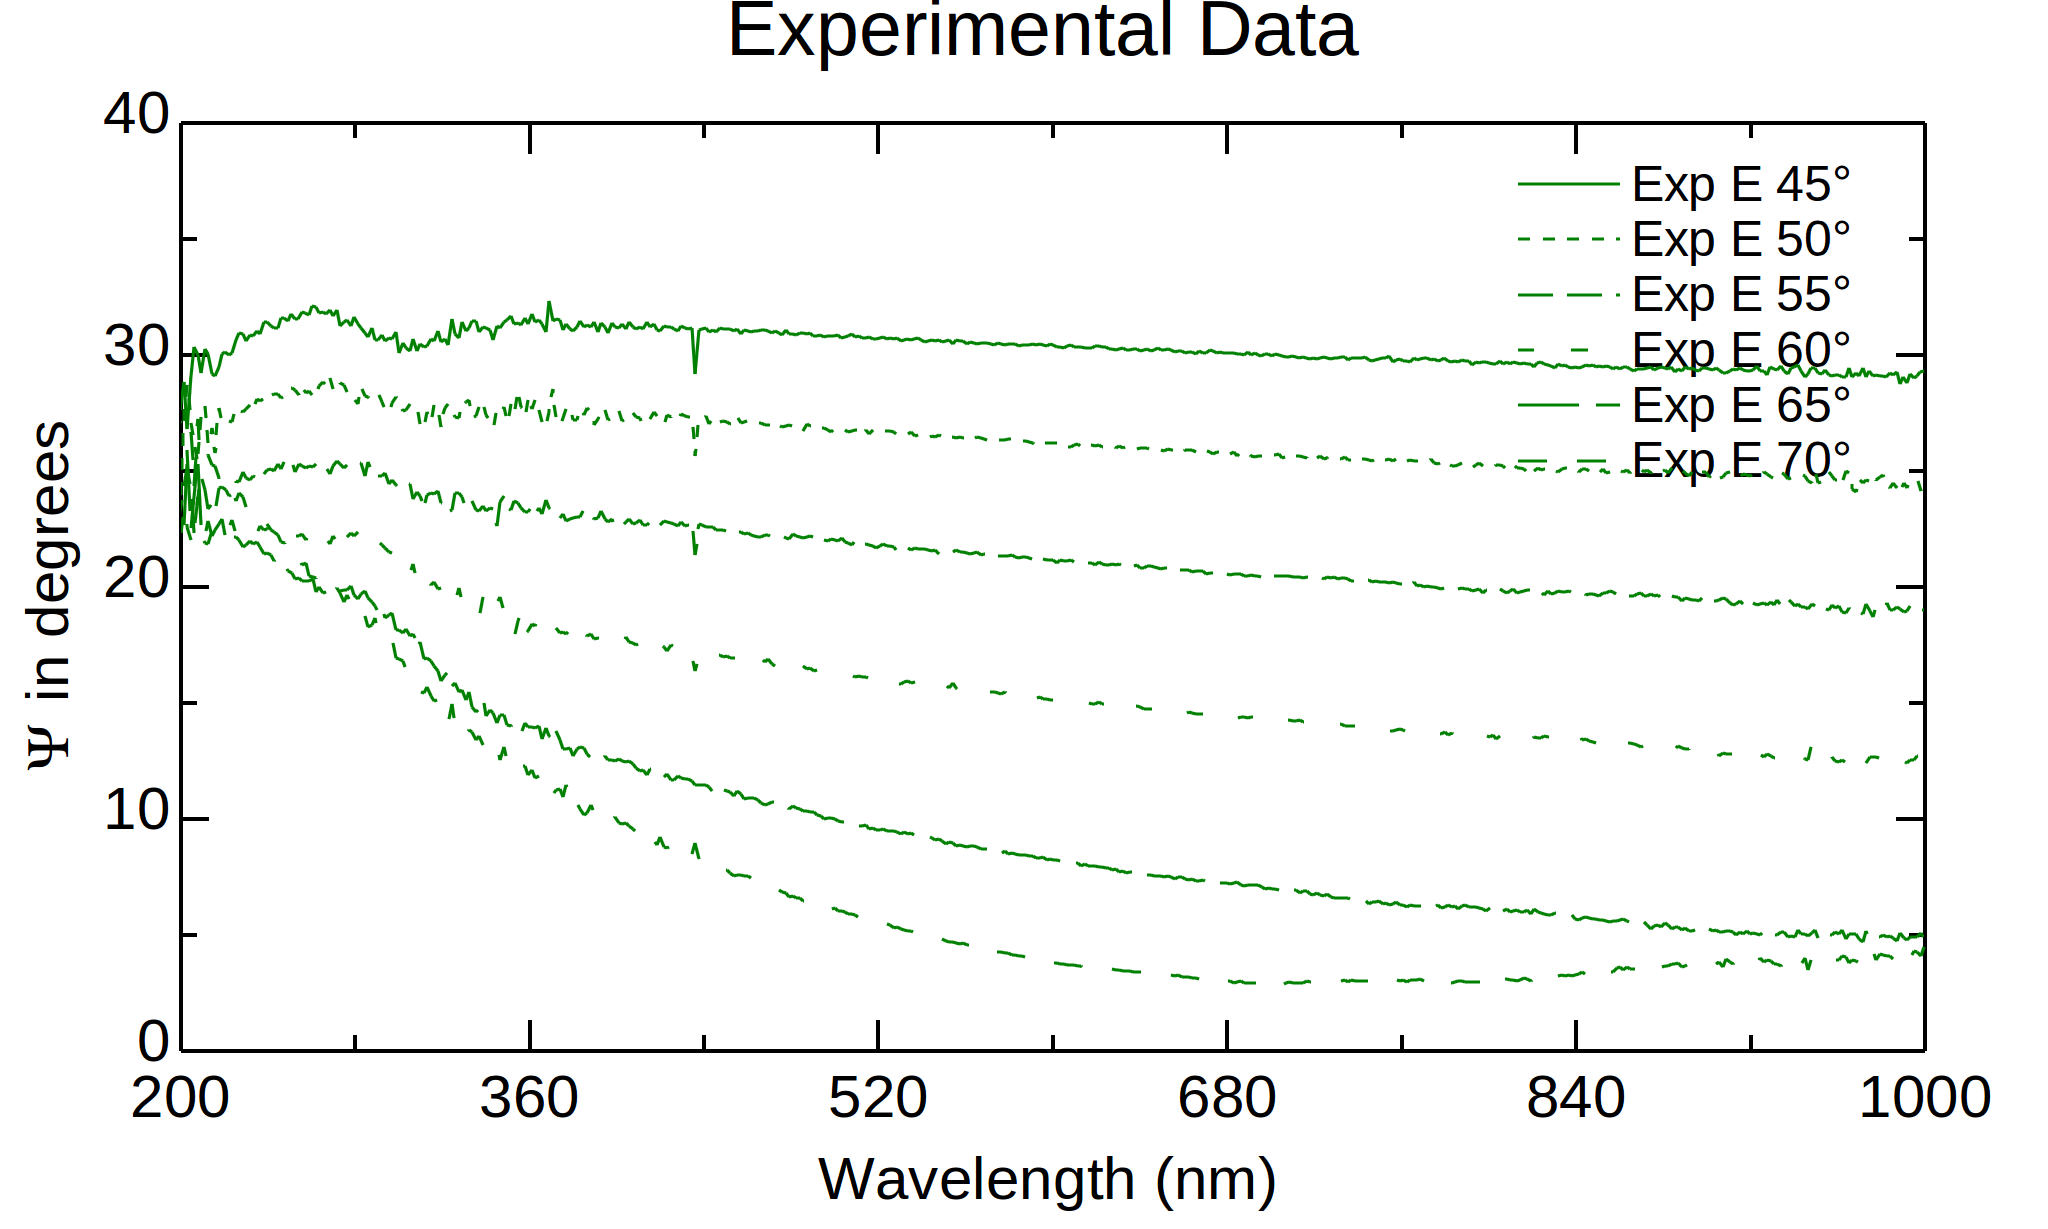
\includegraphics[width=0.5\textwidth]{results/si_ellipsometry_1}}  
  \subfloat[Graph for $\Delta$.\label{fig_si_ellip_2}]{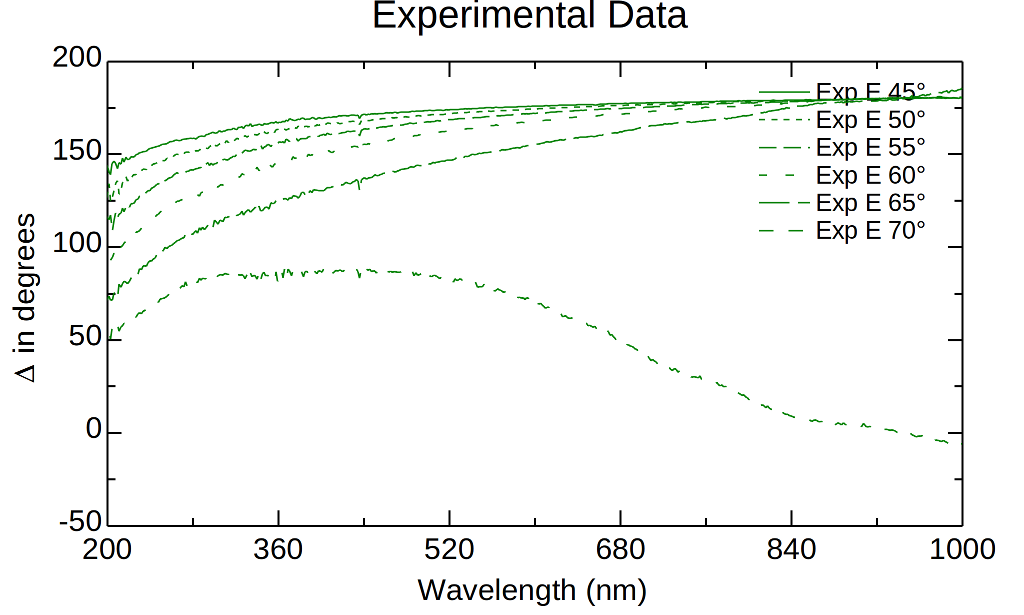
\includegraphics[width=0.5\textwidth]{results/si_ellipsometry_2}}
  \caption[Si ellipsometry.]{Si ellipsometry. Graphs courtesy of Junwei Wei.\label{fig_si_ellip}}
\end{figure}

The data for this sample does not seem to have any meaningful interpretation, just like the gold samples. There appear to be some contribution from the substrate, but not much else.  Reference \cite{PhysRevB.84.165316} demonstrates successful ellipsometric measurements for samples similar to this one. They are consistent with literature and clearly share nothing in common with the results obtained here. The dark grey aspect of the sample may indicate some form of damage to the sample perhaps during annealing or due to environmental aspects or improper handling.

\subsection{XP2SHG and XP2SFG}
Figure \ref{fig_si_shg} was our best SHG run for the Si sample. It is noisy even when compared with the gold samples. It does present the two peak structure but that's where the similarities with previous studies end. Prof. Downer's group reported that XP2SHG enhanced the SHG signal so much that a photon counter was often no longer needed. This was certainly not the case for this sample, with its highest count below 140 photons. The rest of the data produced by this sample was well below this value and did not present even the double peaks.

Figure \ref{fig_si_sfg} is one of only a few SFG runs we did for this sample. Signal intensity was extremely low and looks identical to the substrate contribution.

\begin{figure}[h]
\centering
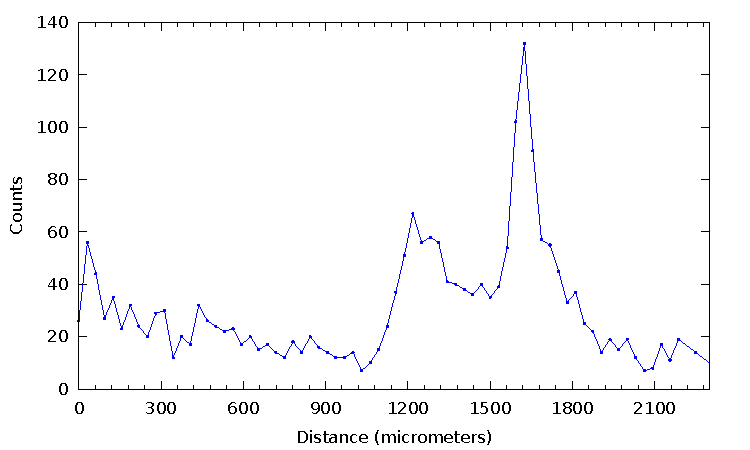
\includegraphics[width=0.85\textwidth]{results/si_shg}
\caption{XP2SHG signal, silicon sample.\label{fig_si_shg}}
\end{figure}

\begin{figure}[H]
\centering
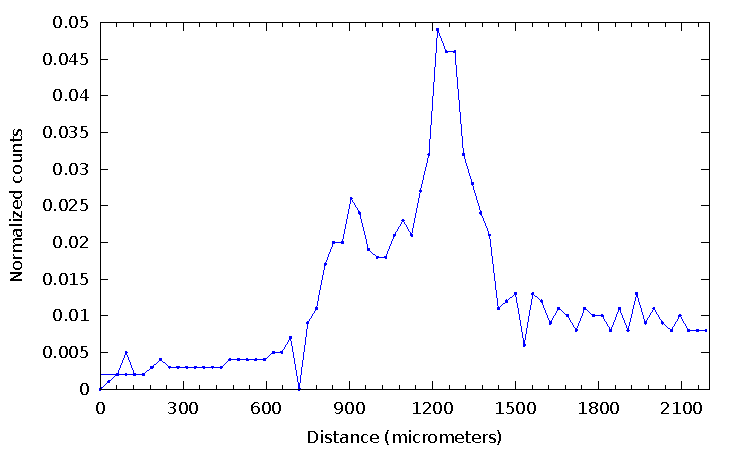
\includegraphics[width=0.85\textwidth]{results/si_sfg_500+800}
\caption{XP2SFG signal, silicon sample.\label{fig_si_sfg}}
\end{figure}

\subsection{Analysis}
I wanted to use this sample as a reference point with the group's previous work, but it became clear from the very beginning that this sample had nothing in common with theirs. After analyzing the linear data we suspected that the sample was most likely damaged in some way. The XP2SHG/SFG runs yielded only a very weak signal compared to the gold samples and to the group's samples. The resulting curves are very inconsistent and ambiguous.

\section{Summary}
We have reviewed all the relevant data for the different samples. Unfortunately the samples were not of good enough quality to yield reliable information. Time constraints and availability did not allow me to obtain different, well characterized, and better samples to redo these measurements. Junwei Wei and Prof. Downer both agreed that these samples had no future for this study and that the data so obtained so far would not yield any meaningful interpretation.

That said, there was a lot learned during this experiment. I review these points and conclude in chapter \ref{chap_conc}.
